\documentclass[12pt]{article}
\usepackage[english]{babel}
\usepackage{float}
\usepackage[utf8]{inputenc}
\usepackage{graphicx}
\usepackage{mathtools}
\usepackage[nottoc]{tocbibind}
\usepackage{tikz}
\usepackage{verbatim}
\usepackage{setspace}
\usepackage{xcolor}
\usepackage{sectsty}
\usepackage[tableposition = top]{caption}


\definecolor{melisa}{RGB}{180,120,20}
\definecolor{hakan}{RGB}{180,0,20}
\definecolor{ugur}{RGB}{120,0,50}

\sectionfont{\color{melisa}}
\subsectionfont{\color{hakan}}
\subsubsectionfont{\color{ugur}}

\setstretch{1.5}

\usepackage{geometry}
 \geometry{
 a4paper,
 total={170mm,257mm},
 left=25mm,
 top=25mm,
 right=25mm,
 bottom=25mm,
 }

\begin{document}


\begin{titlepage}
	\centering

	{\scshape\LARGE Middle East Technical University \par}
	\vspace{0.2cm}
	{\scshape\LARGE EE464 Power Electronics  \par}
	\vspace{3cm}

    
\includegraphics{fiero-logo.png}\par
    {\scshape\LARGE\textit{\textbf{"Turning Coffee into Electricity"}}   \par}
    \vspace{3 cm}
	
	
	{\scshape\LARGE Project 2 Report \par}
	\vspace{1 cm}
	{\Large\itshape \today \par}
		\vspace{0.3 cm}



	
	{\Large\itshape Asena Melisa SARICI -2031284\par}
	\vspace{0.1cm}

	{\Large\itshape Hakan POLAT -\par}
	\vspace{0.1cm}
	
	{\Large\itshape Uğur Can YILMAZ - 2031680  \par}
	\vspace{0.1cm}
	
	
	To be submitted to\par
	{\Large\itshape{Ozan \textsc{KEYSAN}\par}}
	
	

\end{titlepage}


\tableofcontents
\newpage

\newpage
\section{Introduction}

As Fiero Converters, we manufacture 230 V AC to 9 V DC, 10 W Flyback  Converters. This documents shows the detailed pre-manufacturing process of designing, simulating of the converter and the controller of the product. The design to be used in the simulations is provided in figure \ref{fig:design}.





\section{Isolated Converter Simulation}

The design is made using \cite{}. There is snubber in order to reduce the current and voltage stress the MOSFET endures during operation. The resultant effect of the snubber is clearly observed in the simulations as well. The simulations were done synchronously with the implementation and hence the design parameters for the switch, diode and the transformer are taken from the implemented products.

\begin{figure}[H]
    \centering
    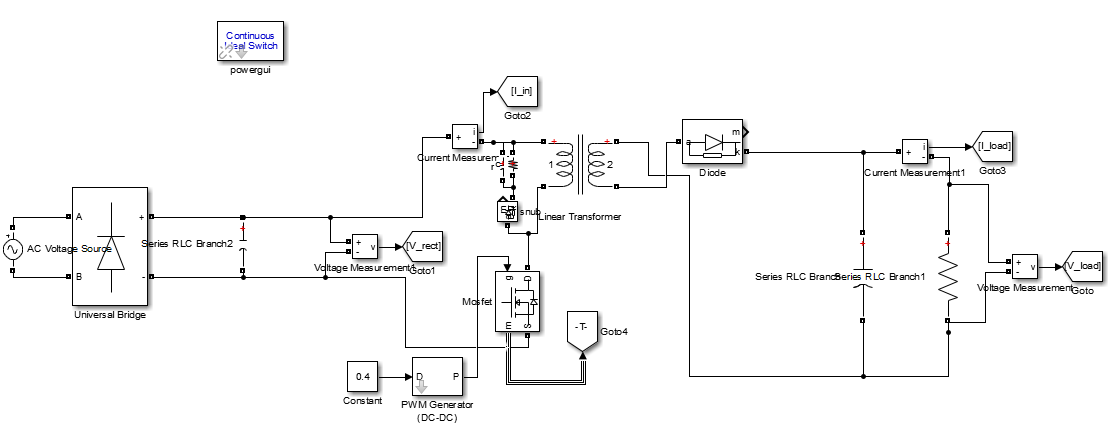
\includegraphics[width=15 cm]{Design}
    \caption{Flyback Design}
    \label{fig:design}
\end{figure}

\subsection{Part I. Steady State Operation of the Converter}

The figures \ref{fig:loadvoltage}, \ref{fig:loadcurrent}, \ref{fig:rectifier}, \ref{fig:display} show the simulation waveforms and the resultant voltage, current and power outputs for the calculated values of maximum duty cycle, turns ratio, reasonable capacitor values and resistance for the ideal case.



\begin{figure}[H]
    \centering
    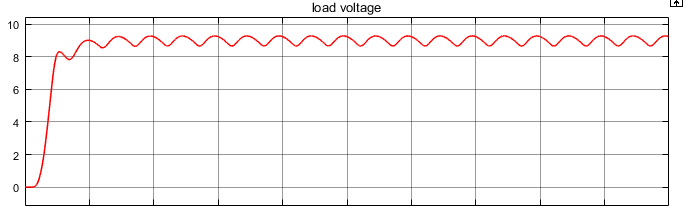
\includegraphics[width=15 cm]{LoadVoltage}
    \caption{Load Steady State Voltage}
    \label{fig:loadvoltage}
\end{figure}

\begin{figure}[H]
    \centering
    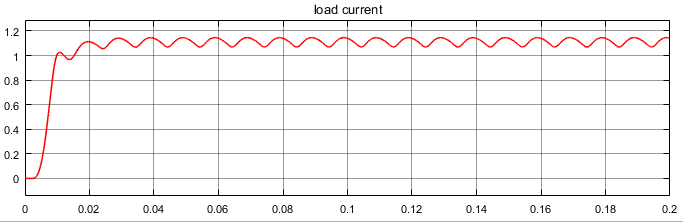
\includegraphics[width=15 cm]{LoadCurrent}
    \caption{Load Steady State Current}
    \label{fig:loadcurrent}
\end{figure}

\begin{figure}[H]
    \centering
    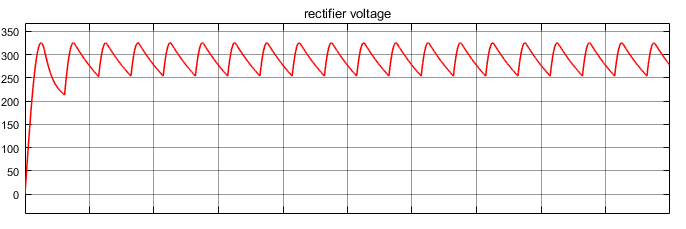
\includegraphics[width=15 cm]{RectifieVoltage}
    \caption{Rectifier Output Voltage at Steady State}
    \label{fig:rectifier}
\end{figure}

\begin{figure}[H]
    \centering
    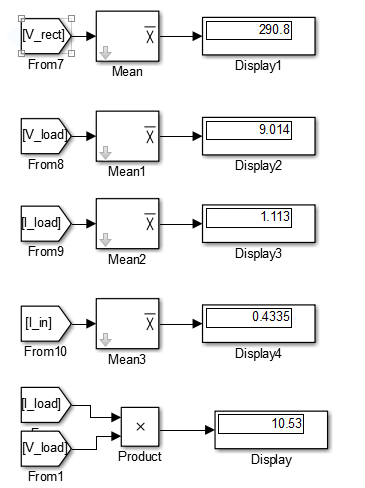
\includegraphics[width=8 cm]{VIvalues}
    \caption{All voltage current display values}
    \label{fig:display}
\end{figure}

Moreover, we have also checked that the switch voltage and current remains in the tolarable range. As expected, the voltage across the switch will be twice the input voltage when it turns off. This can be seen in figure\ref{fig:switch}.

\begin{figure}[H]
    \centering
    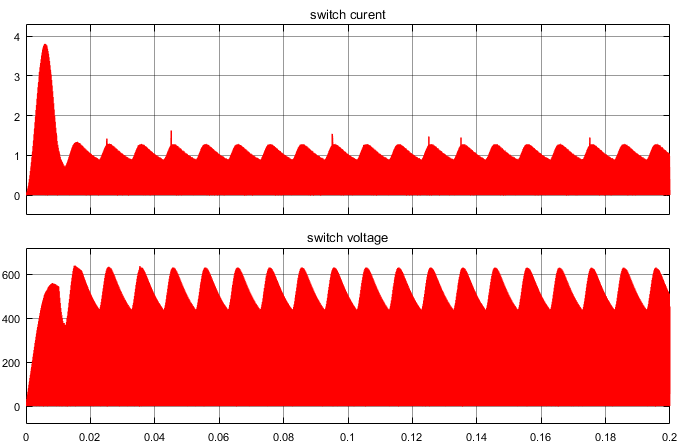
\includegraphics[width=15 cm]{switch_stress_snubbereffect}
    \caption{Current and voltage of the MOSFET during operation}
    \label{fig:switch}
\end{figure}

\subsection{Transformer Design}

Throughout the design procedure we followed the steps of Wurth Transformers.\\
We started our design by defining our specs for the flyback converter which is present in \ref{tab:spec}.
\begin{table}[H]
\centering

\label{tab:spec}
\begin{tabular}{|l|l|}
\hline
$V_{in} $ & $220 V_{ac}$ \\ \hline
$V_{out}$ & 9 V           \\ \hline
$P_{out}$ & 9 W           \\ \hline
\end{tabular}
\caption{Specs of our flyback converter design}
\end{table}


The flyback converter transfers the power stored in the core in off state and the $\Delta I_{lm}$ stays the same since its formula depends on constant values.
\begin{equation*}
    \Delta I_{lm}= \dfrac{V_{in}DT_{s}}{L_{m}}
\end{equation*}
Therefore it is important to let the core have enough discharge time to avoid saturation. Taking these limitations into concideration we decided $D_{max}=0.4$ for the design of the converter.\\
Next step the determination of $V_{in}$ and $V_{out}$. We plan on rectifying the AC voltage to DC using a full bridge diode rectifier and generate a DC voltage using a DC-link capacitor. According to our calculations the $V_{in,dc}$ varies between 300-325 V. As for the $V_{out}$ we will design it for a $V_{out}$ of 10.5 V which also takes the voltage drop in the diode.\\
Knowing $D_{max}$,$V_{in}$ and $V_{out}$ we can calculate the approximate turns ratio using the formula below.
\begin{equation*}
    \dfrac{N1}{N2}=\dfrac{D_{max}}{1-D_{max}}\dfrac{V_{in,min}}{V_{out}}= 19 
\end{equation*}
By recalculating the $D_{max}$ we obtain;

\begin{equation*}
    D_{max}=\dfrac{19}{12+\dfrac{300}{10.5}}=0.399 
\end{equation*}
The next step is to choose the voltage and current rating of the switch. We are using a mosfet since it has a faster switching response and the current on the primary side during on time is low.\\
During off state the $V_{out}$ induces voltage on the primary winding which is $V_{primary}=-V_{d}$.
Therefore the blocking voltage is $V_{switch}=2*V_{in,max}$.
Also a safety margin for the switching peak voltages results in

\begin{equation*}
    V_{sw,max}=2 V_{in,max}+ V_{in,max}=3V_{in,max}=844 V
\end{equation*}
The current rating can be calculated from

\begin{equation*}
    I_{rated,sw}=\dfrac{P_{out}}{V_{out}}*\dfrac{N2}{N1}=0.05A
\end{equation*}
Also in this case a safety margin will be added.\\
The next step is the calculation of the $L_{lm}$ which results in a \%25 ripple in $I_{out}$(Our starting assumption is \%25) 
. Again by using the $\Delta I_{lm}$ equation (this time for off state),

\begin{equation*}
    L_{sekondary}=\dfrac{V_{out}(1-D_{max})}{0.25I_{avg,seconcary}frequency}=\dfrac{10.5(1-0.4)}{0.25*2*62500}=201.6 \mu H
\end{equation*}
If we reflect the found $L_{secondary}$ to primary we get
$L_{primary}=72mH$. \\
After calculating the core inductance we should now consider the $A_{e}$ and $B_{sat}$ of our core. Since the equation
\begin{equation*}
   N_{primary}>\dfrac{L_{primary}I_{primary,max}}{B_{sat}A_{e}}
\end{equation*}
must hold.\\
Our core has an $A_{e}=125mm^2$ and $B_{sat}=0.3T$ by inserting the values to the equation we obtain,
\begin{equation*}
   N_{primary}> 224.64
\end{equation*}
For calculation simplicity and to make the $N_{primary}$
an interger value we selected,
\begin{equation*}
   N_{primary}= 228
\end{equation*}
\begin{equation*}
   N_{secondary}= 12
\end{equation*}
After selecting the turns ratios we should select proper commercial cables. By checking the rated currents, fill factor and our core area we choose the cable types AWG28 and AWG21 for primary and secondary side respectively.

\subsection{Minimum Load Current Within CCM}
To satisfy the continuous conduction mode condition, basically $L_{m}$ current discharge completely. To find minimum load current satisfying this condition, $\Delta I_{lm}$ value should be determined first. Afterwards, half of the $\Delta I_{lm}$ should be equal to the minimum load current reflected to the primary side so that $L_{m}$ current never discharges completely.

\begin{equation*}
    \Delta I_{lm}= \dfrac{V_{in}DT_{s}}{L_{m}}= \dfrac{325V* 0.4*(1/62500)}{72mH} = 0.02888 A
\end{equation*}

Half of the $\Delta I_{lm}$ value is the minimum input current for the CCM. In order to find minimum output current, input current should be reflected. 
\begin{equation*}
    I_{out,min}= \dfrac{\Delta I_{lm}}{2}
\end{equation*}

\begin{equation*}
    I_{out,min}= \dfrac{N_{1}}{N_{2}}*I_{out,min}= 19*0.01444 = 0.27436 A
\end{equation*}
       
\subsection{Efficiency of the Converter}

In this section, efficiency of the converter will be calculated for different loading conditions. Efficiency equation of the converter is basically given below. 

\begin{equation*}
    \eta = \dfrac{V_{out}*I_{out}}{V_{in}*I_{in}}
\end{equation*}      
For full load condition :
       
\begin{equation*}
    \eta_{100} = \dfrac{V_{out}*I_{out}}{V_{in}*I_{in}}=\dfrac{9.01*1.112}{316.5*0.04564}= \dfrac{9.4}{12}= 75 \%
\end{equation*} 

For \%75 load condition :
       
\begin{equation*}
    \eta_{75} = \dfrac{V_{out}*I_{out}}{V_{in}*I_{in}}=\dfrac{9.01*0.85}{321*0.037}= \dfrac{7.87}{11.8}= 66 \%
\end{equation*} 

For \%50 load condition :
       
\begin{equation*}
    \eta_{50} = \dfrac{V_{out}*I_{out}}{V_{in}*I_{in}}=\dfrac{9.01*0.74}{321*0.032}= \dfrac{6.7}{10.2}= 64 \%
\end{equation*} 

For \%25 load condition :
       
\begin{equation*}
    \eta_{25} = \dfrac{V_{out}*I_{out}}{V_{in}*I_{in}}=\dfrac{9.01*0.64}{321*0.029}= \dfrac{5.98}{9.3}= 64 \%
\end{equation*} 


\subsection{Preliminary Component Selection}

In this section, selected components to be used in the implementation will be given. 

For the mosfet ;

\begin{equation*}
    V_{sw,max}=2 V_{in,max}+ V_{in,max}=3V_{in,max}=844 V
\end{equation*}
The current rating can be calculated from

\begin{equation*}
    I_{rated,sw}=\dfrac{P_{out}}{V_{out}}*\dfrac{N2}{N1}=0.05A
\end{equation*}
According to current and voltage ratings, Toshiba 2SK1119 MOSFET is chosen.It has 1000V drain to source voltage rating and 4A drain current capacity.

Also in the simulation, frequency is chosen to be 62500 Hz. Selected MOSFET is quite capable of working in this frequency.

For the diode located at the secondary side, MBRA320T3G is chosen. Rating of the secondary side current is 1.1A which is lower than 3A current rating of the diode. Also breakdown voltage of the diode is 20V which is quite sufficient for the operation. 

As a result of calculations in the previous parts, 680 $\mu$F capacitor with 1200V voltage rating will be placed to output of diode rectifier. Another 4.7mF capacitor will placed to the output of the converter.  

For the core selection, we have visited Konya Sokak and due to lack of datasheet, we have been informed by the seller. According to him, our core has an $A_{e}=125mm^2$ and $B_{sat}=0.3T$. We made transformer design according to this information. 

\section{Controller Design}

This part contains the desired control design for our flyback converter. The controller is chosen to be type 2 controller with a schematic shown in figure \ref{fig:controller}.
\begin{figure}[H]
    \centering
    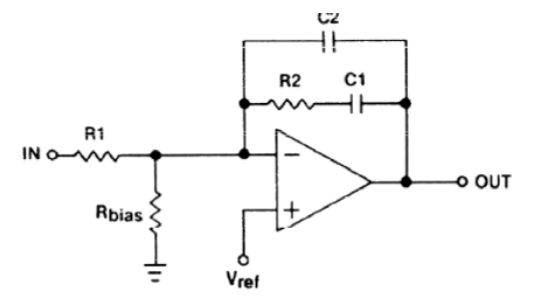
\includegraphics[width=15 cm]{controller}
    \caption{Type 2 Controller}
    \label{fig:controller}
\end{figure}

\subsection{Part 1. Controller Transfer Function}

The transfer function for the controller is:

\begin{equation*}
    \Tilde{v_{c}}/\Tilde{v_{o}}=Z_{feedback}/Z_{input}
\end{equation*}

COnsider that the input and output voltages contain DC and ACcomponents, while the reference is DC. In order to derive the transfer function, consider the AC components:


\begin{equation*}
    Z_{feedback}=1/sC_2// (R_2 +1/sC_1)\\
\end{equation*}
\begin{equation*}
Z_{input}=R_1 R_{bias}/(R_1 + R_{bias})
\end{equation*}

This yield the following transfer function:

\begin{equation*}
T_c(s)=\dfrac{R_1+R_{bias}}{R_1 R_{bias} }\cdot \dfrac{1}{C_2}\cdot \dfrac{s+1/(R_1 C_1)}{s(s+(C_1+C_2)/R_2C_1C_2)}
\end{equation*}

Here, we observe that the controller is a compensator function. It is in our control to make it either a lead or lag compensator. For stability, we need an increase in the phase margin of our close loop system. Hence, we desire the controller to add a phase lead (boost). Therefore, we need to place a zero before a pole so that first an incline in the phase occurs. The general bode plot for the controller transfer function is provided in figure \ref{fig:bode}, we see that the zero is placed before the pole. 

\begin{figure}[H]
    \centering
    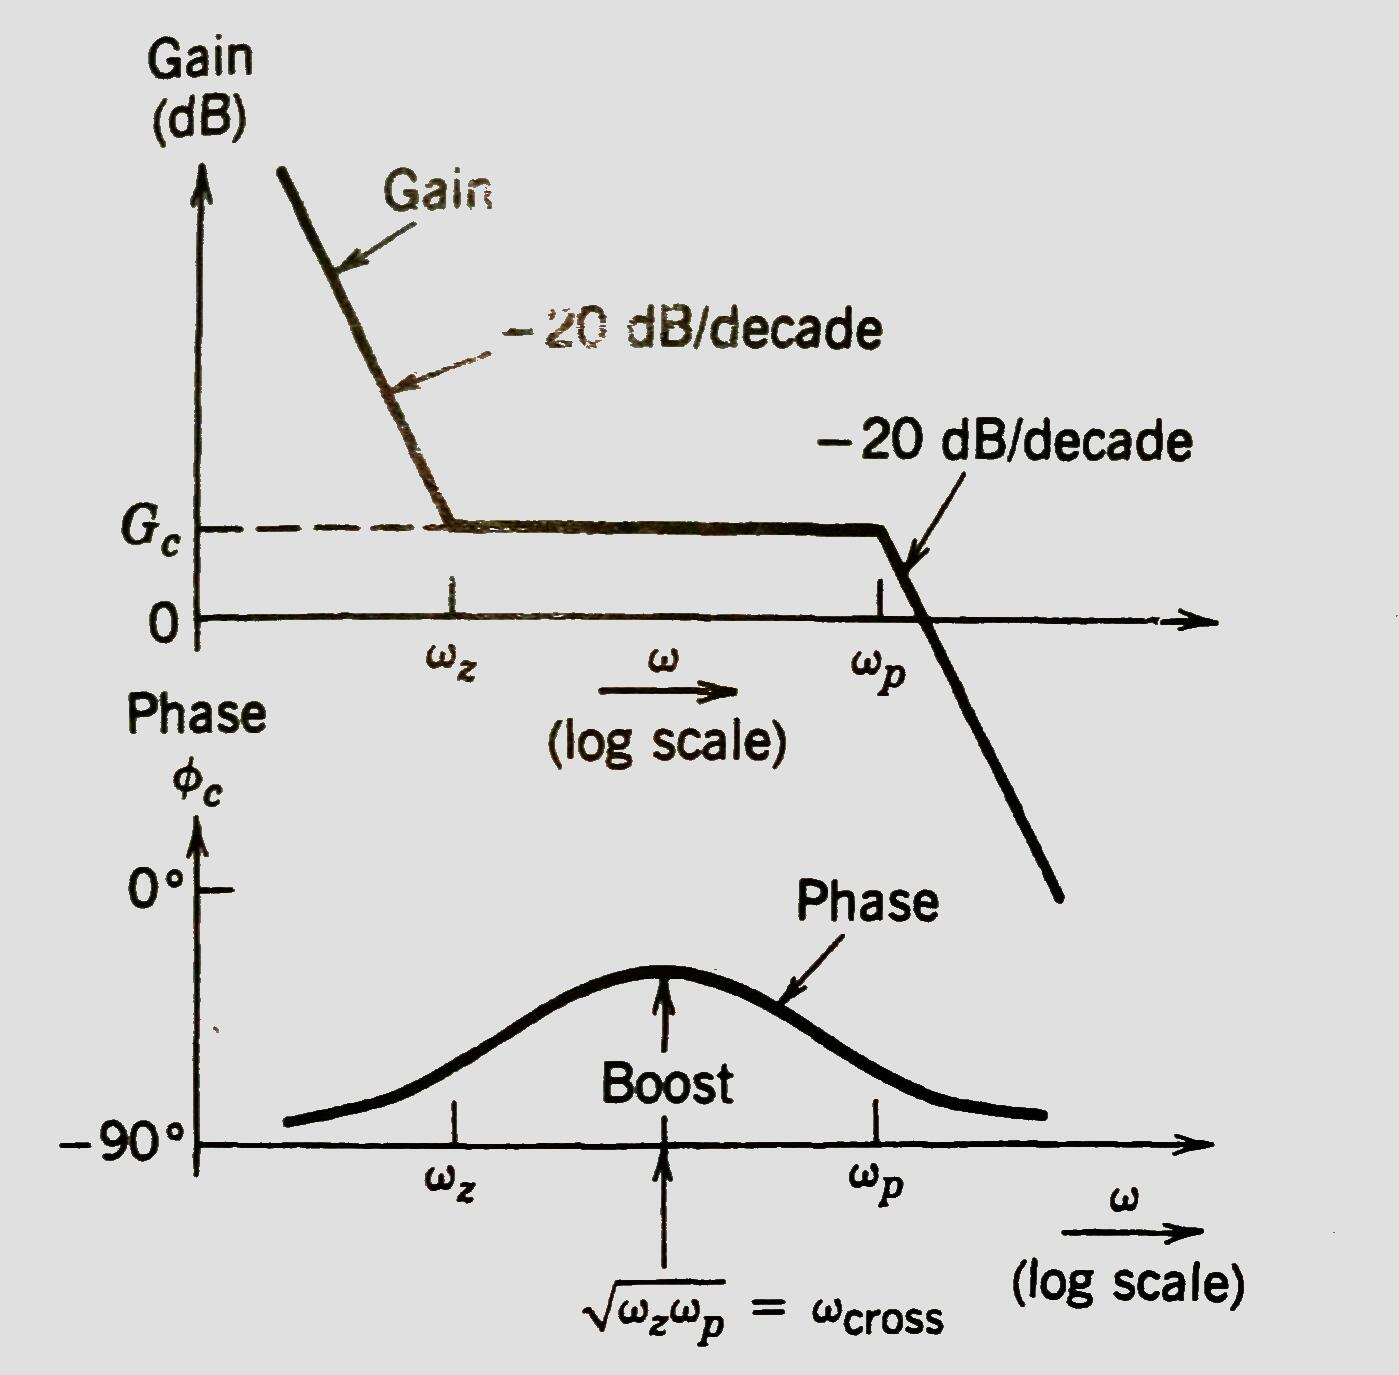
\includegraphics[width=10 cm]{bode}
    \caption{Type 2 Controller Bode Plot}
    \label{fig:bode}
\end{figure}

\subsection{Controller Computer Simulation -b and c-}
The bode plot for type 2 controller is simulated as seen in figure\ref{fig:controller}

\begin{figure}
    \centering
    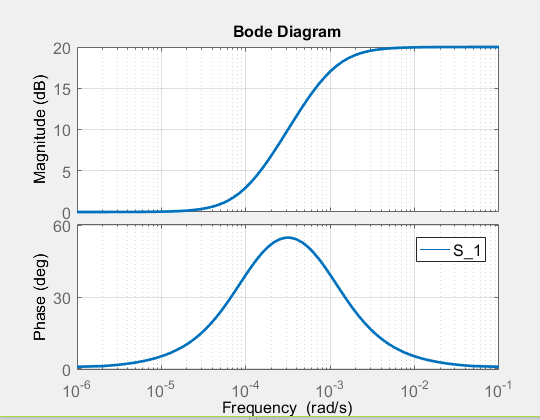
\includegraphics{controllerd}
    \caption{Controller designed for the plant}
    \label{fig:controller}
\end{figure}

This controller was designed for the flyback converter. Since the transfer function for a flyback isa nonlinear one, first a system identification is applied on the converter. Then, not being sure whether this system is fine, literature is researched and an application noteof texas instruments(http://www.ti.com/lit/an/slua086/slua086.pdf) is found explaining in detail of how to select the necessary parameters.



The rightmost zero (the one closer to the unstable region) is found from:
\begin{equation}
    \omega_{rhz}=\dfrac{N V^2_{in}}{R_{out}L_p(V_{in} +N V_{out}) }
    \label{1}
\end{equation}

Using the measured inductance of our core, this yields a zero around $0.5 10^{-4}$ and according to the document, this zero determines the maximum crossover frequency. Taking this value as our crossover frequency, one zero and one pole is selected. $\omega_{z}=0.0001 and \omega_{p}=0.001$. 

Once again the document suggests that for compensation, high gain at low frequencies is needed. Hence,the gain is selected as 10. For very low frequencies, the gain contribution of the controller is 1. 

The closed loop control works fine and the system settles at the very desired point. The results are shown in \ref{fig:controlled}  and \ref{fig:controllerout}.
\begin{figure}[H]
    \centering
    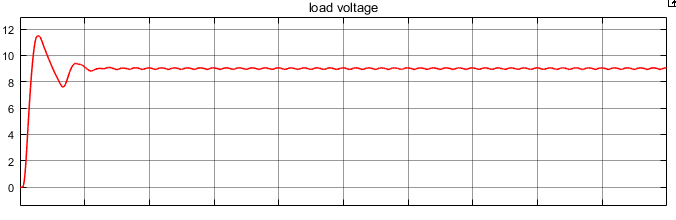
\includegraphics[width=14cm]{controlledvoltage}
    \caption{Controller output voltage}
    \label{fig:controlled}
\end{figure}

\begin{figure}[H]
    \centering
    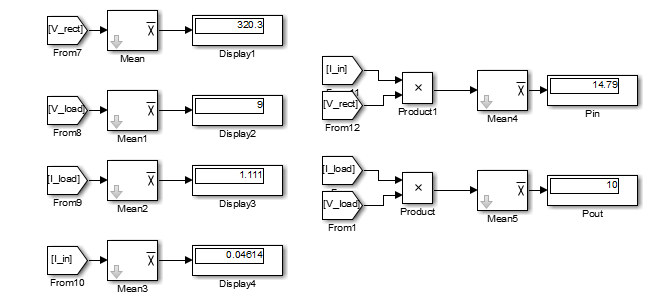
\includegraphics[width=14cm]{controlledoutput}
    \caption{Controller output values}
    \label{fig:controllerout}
\end{figure}

\section{Load and input Change Adaptation}

The controller behaves very quick and compensated to the load changes as seen in \ref{fig:d1} and \ref{fig:d2}.

\begin{figure}[H]
    \centering
    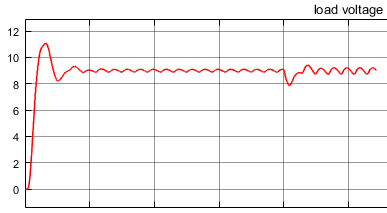
\includegraphics[width=14cm]{d1}
    \caption{Controller output voltage for load increase}
    \label{fig:d1}
\end{figure}

\begin{figure}[H]
    \centering
    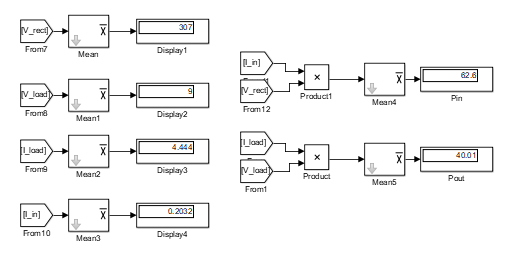
\includegraphics[width=14cm]{d2}
    \caption{Controller output values for load increase}
    \label{fig:d2}
\end{figure}

And when the Ac voltage input is decreased by 10 percent from its nominal value, the controller is still able to keep the output at 9 V.

\begin{figure}[H]
    \centering
    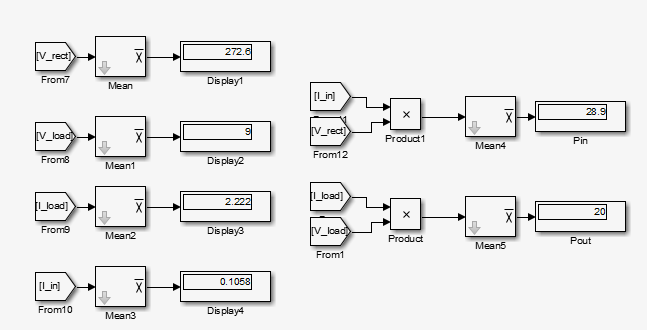
\includegraphics[width=14cm]{d3}
    \caption{Controller output voltage for input decrease 200V AC}
    \label{fig:d1}
\end{figure}

\begin{figure}[H]
    \centering
    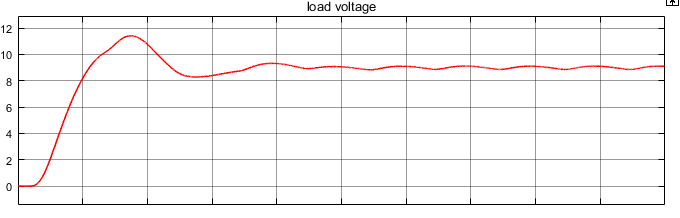
\includegraphics[width=14cm]{d4}
    \caption{Controller output values for input decrease 200V AC}
    \label{fig:d2}
\end{figure}

\section{Discussion}

This controller performs very quick and the output oscillation is acceptable. At the very beginning it has an overshoot but this overshoot settles quickly. The controller is capable of adjusting to both input and output changes. 

\begin{figure}
    \centering
    \includegraphics{controllerreoınse}
    \caption{Frequency response of the flyback from system identification}
    \label{fig:fr}
\end{figure}

Looking at the frequency response \ref{fr} and the crossover frequency we have calculated from the document base equation \ref{1}, we see that the derived and simulated values do fit. And we observe that the controller works nice.

\end{document}
